%!TEX root = MemoireZelliges.tex

\chapter{Étude physique d'un zellige miel (\bdx{6531})}
%======================================================================

\section{Description -- État de surface}
%----------------------------------------------------------------------

Cet échantillon, de forme parallélépipédique, est une 
pièce de céramique chanfreinée, comportant une glaçure miel 
(\fref{dessin:6531}). Il provient du \PaM (\siecle{17}) de Meknès.

\begin{itemize}
  \item \DimText : \SI{50x50x25}{\mm}
  \item \emph{Masse} : \SI{83.5}{\g}
\end{itemize}

\begin{figure}[htb]
  \begin{minipage}[b]{3.9cm}
    \centerfloat
    \vspace*{0pt}
    % Dessin de l'échantillon : Vue de dessus
    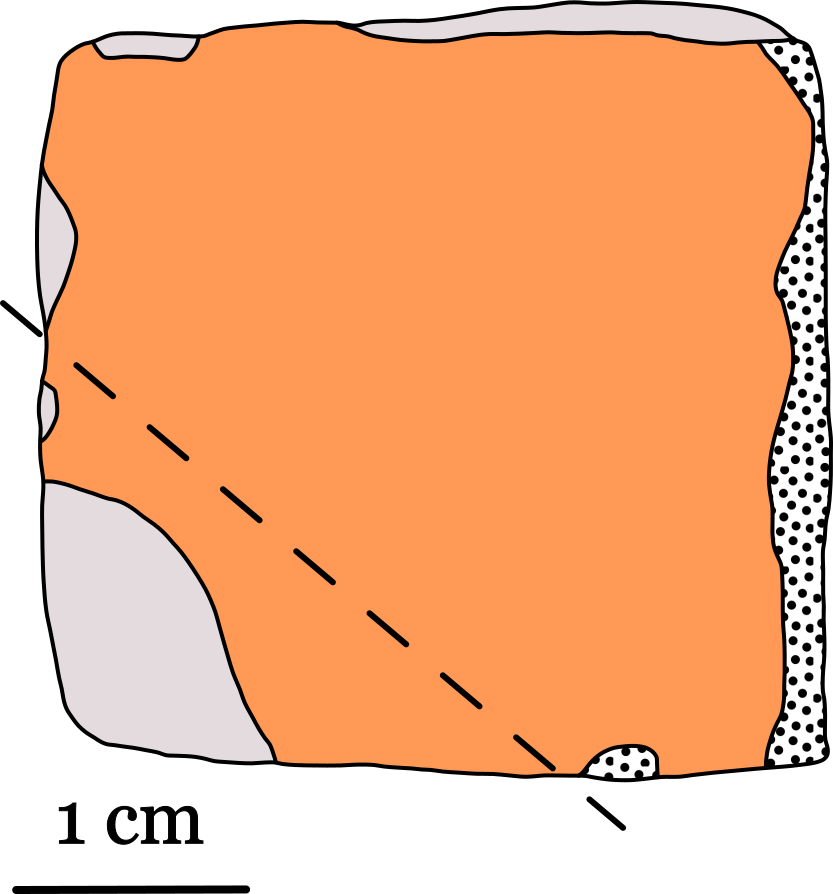
\includegraphics[scale=0.17]{PaM_BDX6531_dessus}
    \subcaption{Vue de dessus \label{dessin:6531_dessus}}

    \bigskip

    % Dessin de l'échantillon : Coupe
    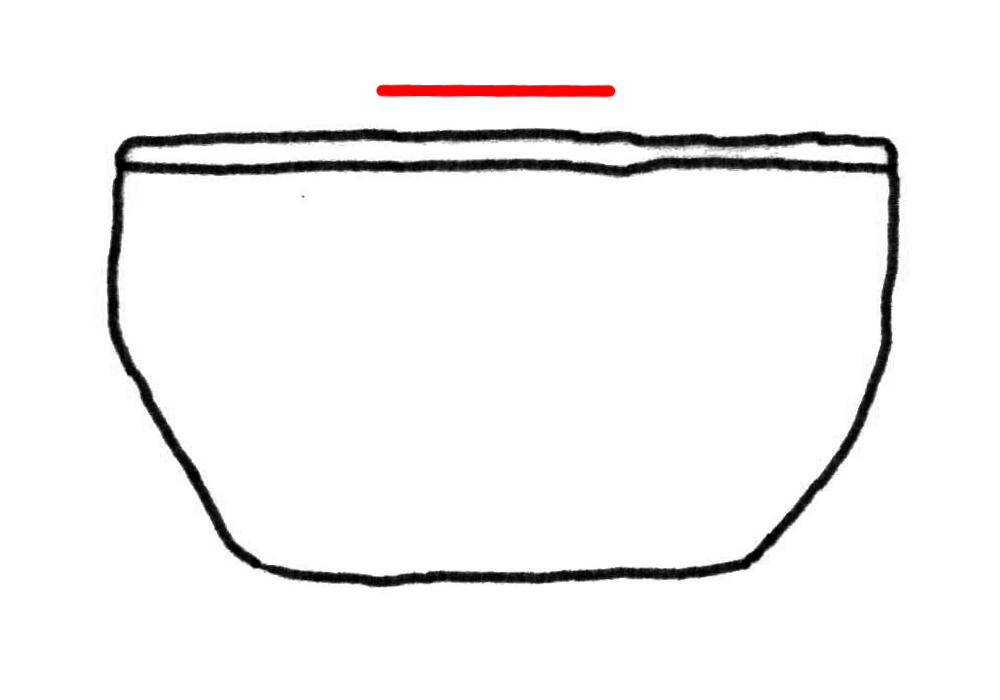
\includegraphics[scale=0.17]{PaM_BDX6531_coupe}
    \subcaption{Vue en coupe \label{dessin:6531_coupe}}
  \end{minipage}%
  \qquad%
  \begin{minipage}[b]{4.1cm}
    \centerfloat
    \vspace*{0pt}
    % Dessin de l'échantillon : Lame
    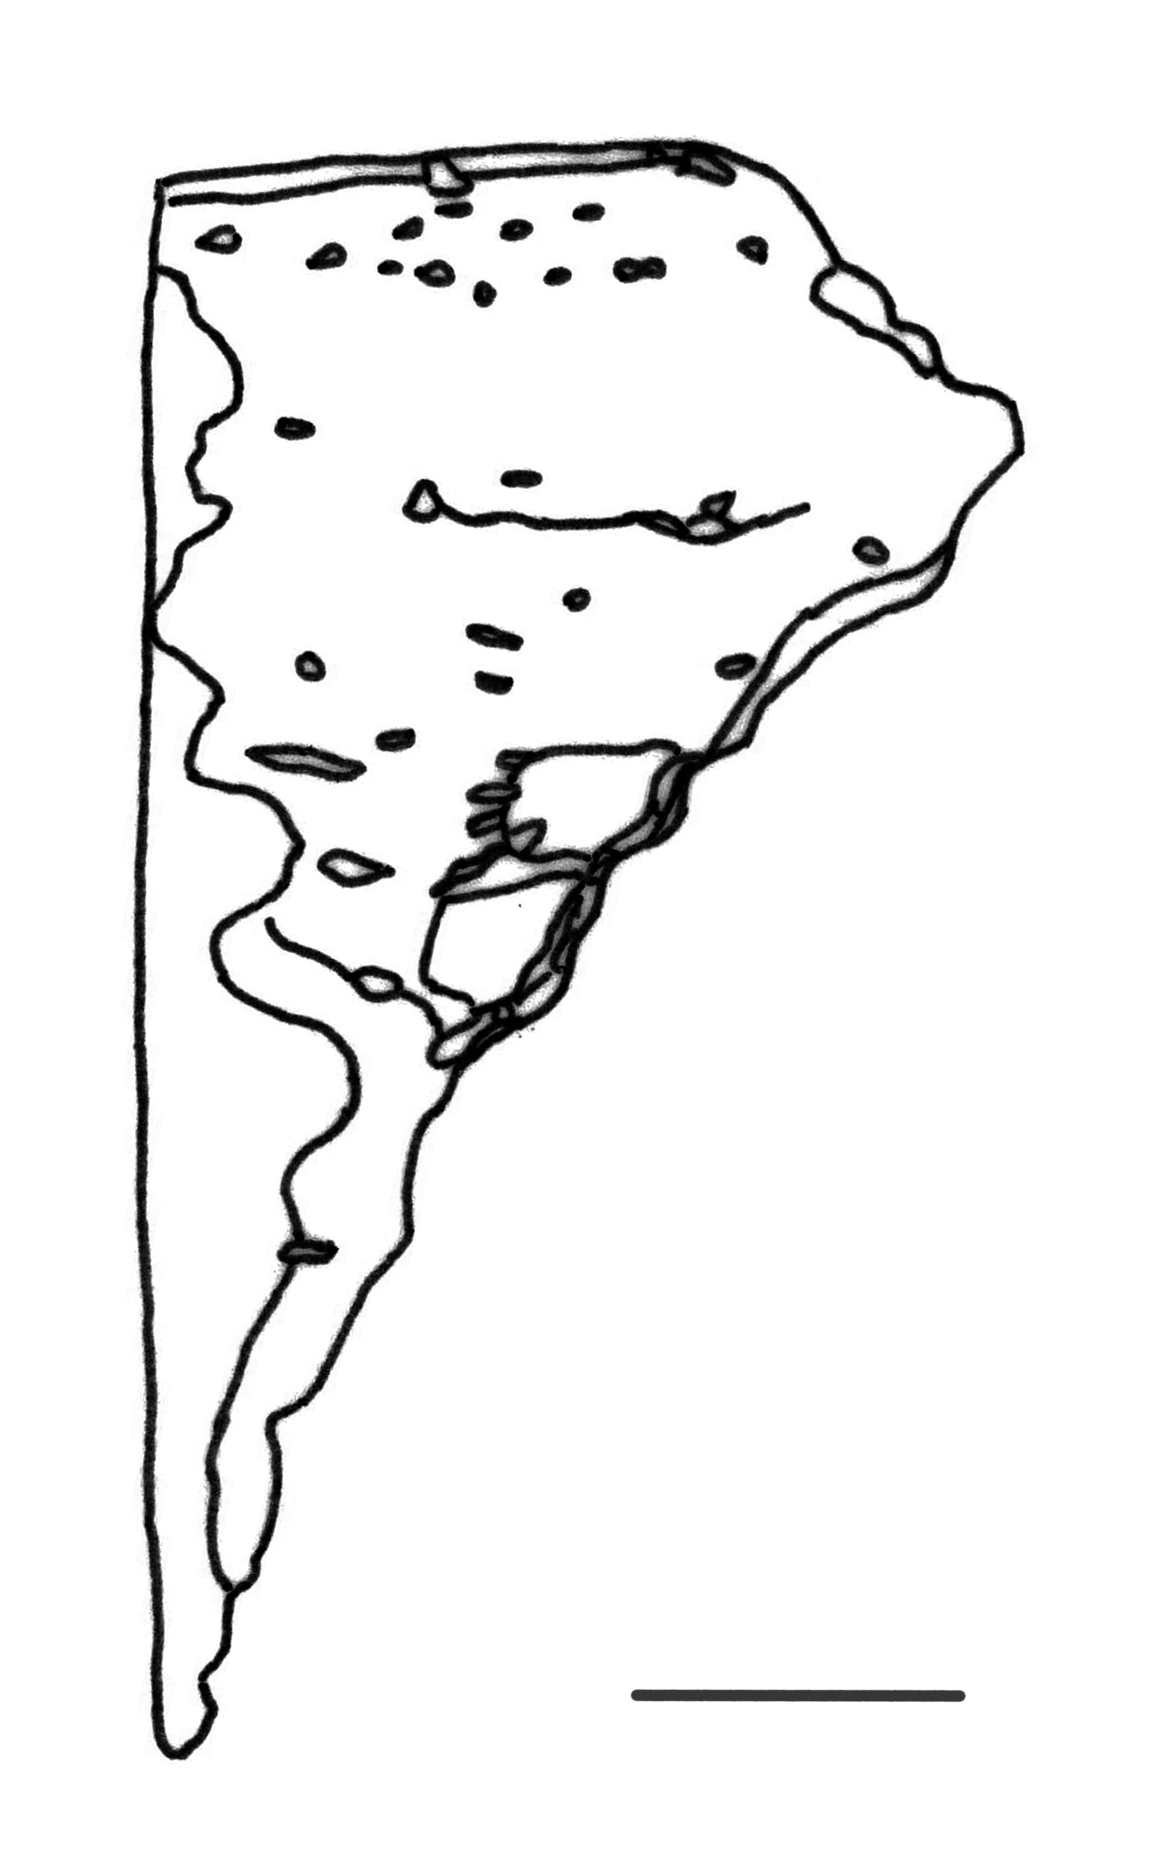
\includegraphics[scale=0.17]{PaM_BDX6531_lame}
    \subcaption{Lame étudiée \label{dessin:6531_lame}}
  \end{minipage}
  \qquad%
  \begin{minipage}[b]{3.2cm}
    \vspace*{0pt}

    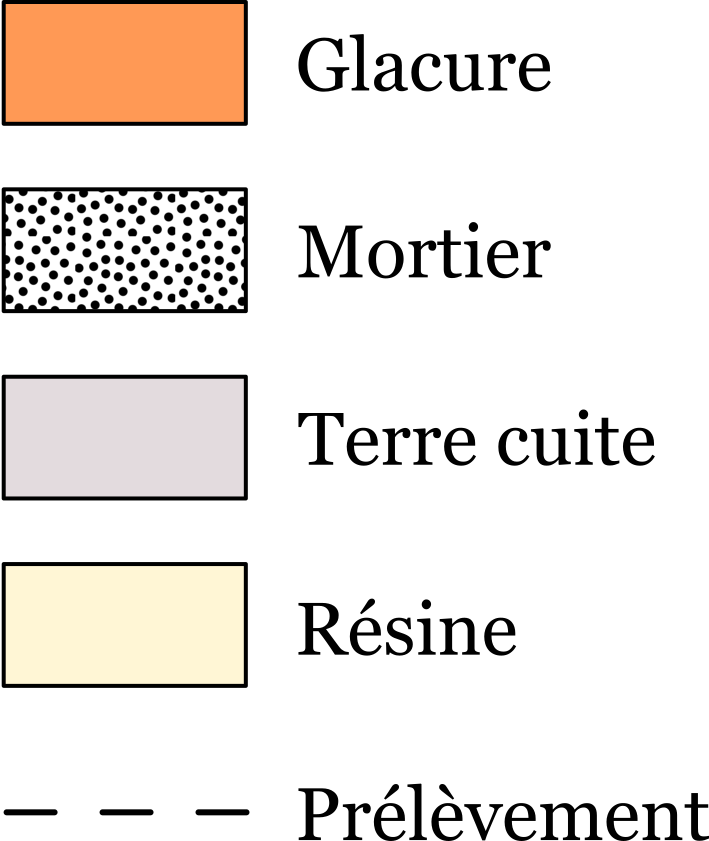
\includegraphics[scale=0.17]{PaM_BDX6531_legende}

    \bigskip
  \end{minipage}
  \caption[\bdx{6531}]{\legendeD.}
  \label{dessin:6531}
\end{figure}

L'observation de la surface de la glaçure (\fref{surf:6531}) montre 
qu'elle contient des bulles, des picots et des cristaux non fondus.

Le support de terre cuite est de couleur ocre rosé, de granulométrie
fine, assez poreux et contient de nombreuses inclusions de tailles et
de couleurs variées.

\begin{figure}[htb]
  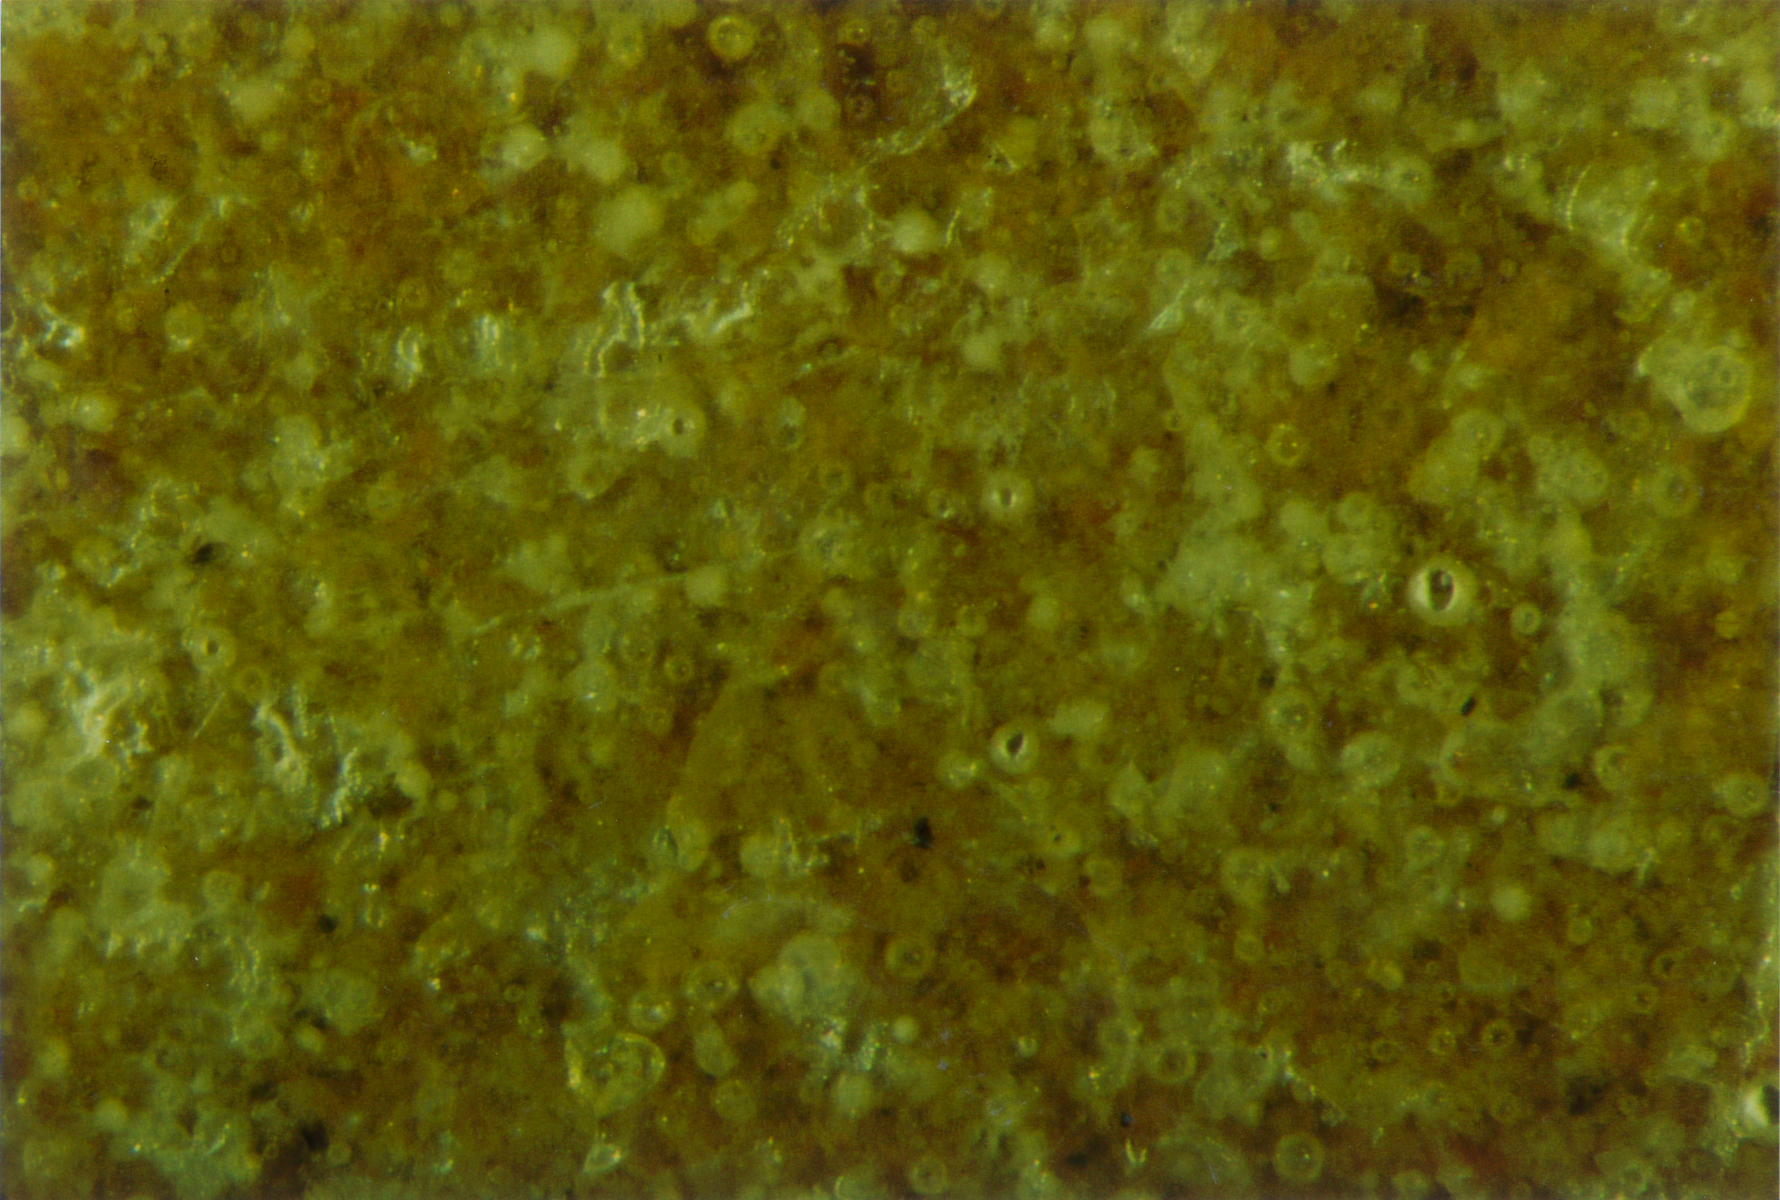
\includegraphics[width=\textwidth]{PaM_BDX6531_Surf}
  \caption[\bdx{6531}\ -- État de surface de la glaçure]
          {\legendeD.
           État de surface de la glaçure 
           (Gr=30, \zone{\sim4.3x3.2}{\mm}). Elle contient des bulles, 
           des picots et des cristaux non fondus.}
  \label{surf:6531}
\end{figure}


\section{Étude de la couleur}
%----------------------------------------------------------------------

\subsection{Identification des ions chromogènes}
%~~~~~~~~~~~~~~~~~~~~~~~~~~~~~~~~~~~~~~~~~~~~~~~~~~~~~~~~~~~~~~~~~~~~~~
\begin{figure}[htb]
  \begin{plotspectre}
    \addplot [thick, Orange] 
       table [x=lambda, y=6531gla] {\gladata} ;
    \addlegendentry{glaçure miel}
    \addplot [thick, FireBrick] 
       table [x=lambda, y=6531tc] {\tcdata} ;
    \addlegendentry{terre cuite}

    \begin{scope}[<-, >=stealth, shorten <=5pt, thin]
      \node (Fe) at (410.00, 0.45) {\ch{Fe^3+}} ;
      \node (qm) at (540.00, 0.30) {?} ;
      \draw (380.00, 0.73) |- (Fe.north) ;
      \draw (440.00, 0.61) |- (Fe.north) ;
      \draw (540.00, 0.46) |- (qm.north) ;
    \end{scope}
  \end{plotspectre}
  \caption[\bdx{6531}\ -- Spectres d'\AO en mode réflexion diffuse 
           de la glaçure et de la terre cuite]
          {\legendeD.
           Spectres d'\AO en mode réflexion diffuse de la glaçure et 
           de la terre cuite. La glaçure présente des absorptions vers 
           \SIlist{380;440}{\nm}, correspondant au \ch{Fe^3+}.}
  \label{spectre:6531}
\end{figure}

Le spectre d'\AO en mode réflexion diffuse de la glaçure 
(\fref{spectre:6531}) présente une forte absorption à \SI{370}{\nm} 
et un épaulement à \SI{440}{\nm} attribuables au \ch{Fe^3+}. La terre 
cuite présente des épaulements à \SIlist{380;440}{\nm}, probablement 
attribuables au \ch{Fe^3+} ainsi qu'une bande d'absorption vers 
\SI{550}{\nm} qui n'a pu être attribuée.

\subsection{Mesure physique de la couleur}
%~~~~~~~~~~~~~~~~~~~~~~~~~~~~~~~~~~~~~~~~~~~~~~~~~~~~~~~~~~~~~~~~~~~~~~
Le \tref{saotab:6531} regroupe les coordonnées chromatiques, 
correspondant aux espaces \Yxy et \Lab, calculées à partir des 
spectres d'\AO de la glaçure et de la terre cuite.

La longueur d'onde dominante de la glaçure (\SI{579.24}{\nm}) 
correspond au domaine du jaune \autocite{Kelly_1976}. la couleur 
de la glaçure est foncée (réflectance $\CIEY=\num{22.955}$) et assez 
saturée ($\Pe=\SI{43.65}{\percent}$). La \tref{saotab:6531} montre 
la localisation des coordonnées chromatiques de la glaçure dans les 
espaces \Yxy et \Lab. La couleur de la terre cuite se situe dans le 
domaine du jaune orange. Elle est assez claire, étant donnée sa 
réflectance ($\CIEY=\num{38.927}$).

\begin{table}[hbt]
  \caption[\bdx{6531}\ -- Coordonnées chromatiques et longueur d'onde 
           dominante]
          {\legendeD.
           Coordonnées chromatiques dans les systèmes \Yxy et \Lab 
           et longueur d'onde dominante (illuminant D65, \ang{2},
           \SIrange{400}{700}{\nm}). (\up{\dag}\,\cite{Kelly_1976})}
  \label{saotab:6531}
  \begin{chrotab}
      \chrolgna{Glaçure}{579.24}{43.65}
               {22.955}{0.398}{0.400}
               {55.026}{4.617}{27.619} &
      \chrolgnb{jaune foncé}{Jaune}{575}{580}{}
               % {\footnotemark{}}
    \tabularnewline
      \chrolgna{Terre cuite}{583.07}{27.15}
               {38.927}{0.372}{0.366}
               {68.698}{8.231}{19.231} &
      \chrolgnb{jaune orange clair}{Jaune-Orange}{580}{585}{}
               {\footnotemark{}}
    \tabularnewline
  \end{chrotab}
\end{table}
% \addtocounter{footnote}{-1}
% \footnotetext{\autocite{Kelly_1976}}
% \addtocounter{footnote}{+1}
% \footnotetext{\autocite{Kelly_1976}}

\begin{figure}[htb]
  \newcommand{\samplename}{6531gla}
  \newcommand{\samplecolor}{Orange}
  \begin{minipage}[t]{0.37\paperwidth}
    \begin{plotYxy}
      \plotYxyPaV ;
      \plotYxyIlluminant ;
      \plotYxySample{\samplename}{\samplecolor} ;
      \plotYxyLigne{\samplename} ;
      \plotYxyAnnot{\samplename}{south west} ;
    \end{plotYxy}
    \subcaption[Espace \trichro \Yxy]
               {Espace \trichro \Yxy. La longueur d'onde 
                dominante de la glaçure est de \SI{594.38}{\nm} 
                et correspond au domaine des oranges.}
  \end{minipage}%
  \qquad%
  \begin{minipage}[t]{0.37\paperwidth}
    \begin{plotLab}
      \plotLabSample{\samplename}{\samplecolor} ;
    \end{plotLab}
    \subcaption{Espace \trichro \Lab}
  \end{minipage}%
  \caption[\bdx{6531}\ -- Analyse chromamétrique de la glaçure]
          {\legendeD. Analyse chromamétrique de la glaçure.}
  \label{colorfig:6531}
\end{figure}


\section{Étude de la texture de la glaçure et de la terre cuite sur 
         une section polie}
%----------------------------------------------------------------------

\subsection{Observation en lumière naturelle}
%~~~~~~~~~~~~~~~~~~~~~~~~~~~~~~~~~~~~~~~~~~~~~~~~~~~~~~~~~~~~~~~~~~~~~~
\begin{figure}[htb]
  \begin{minipage}[t]{0.48\textwidth}
    \centerfloat
    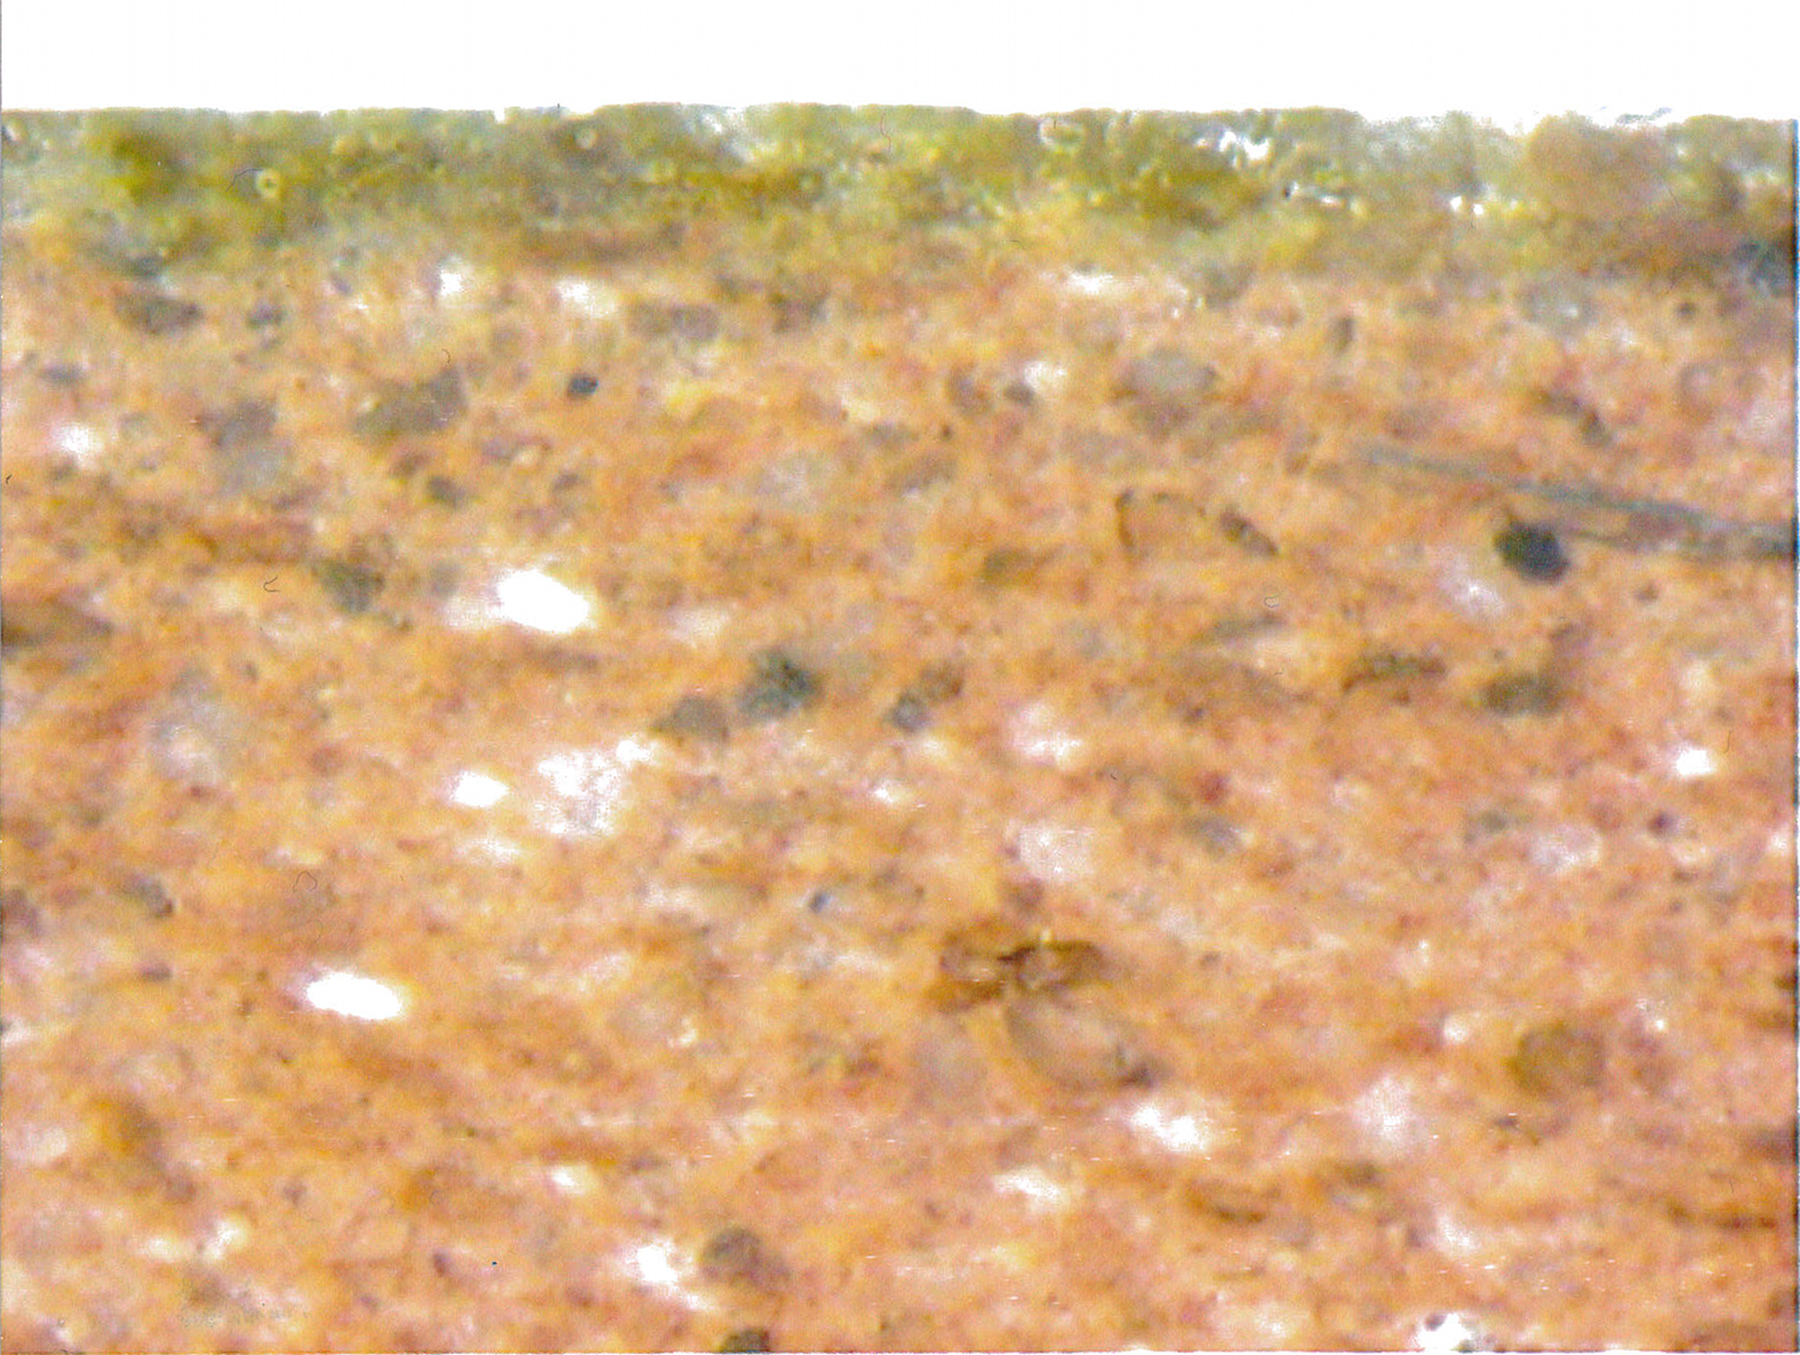
\includegraphics[width=\textwidth]{PaM_BDX6531_LN}%
    \subcaption{Lumière naturelle \label{texture:6531_LN}}
  \end{minipage}%
  \hfill%
  \begin{minipage}[t]{0.48\textwidth}
    \centerfloat
    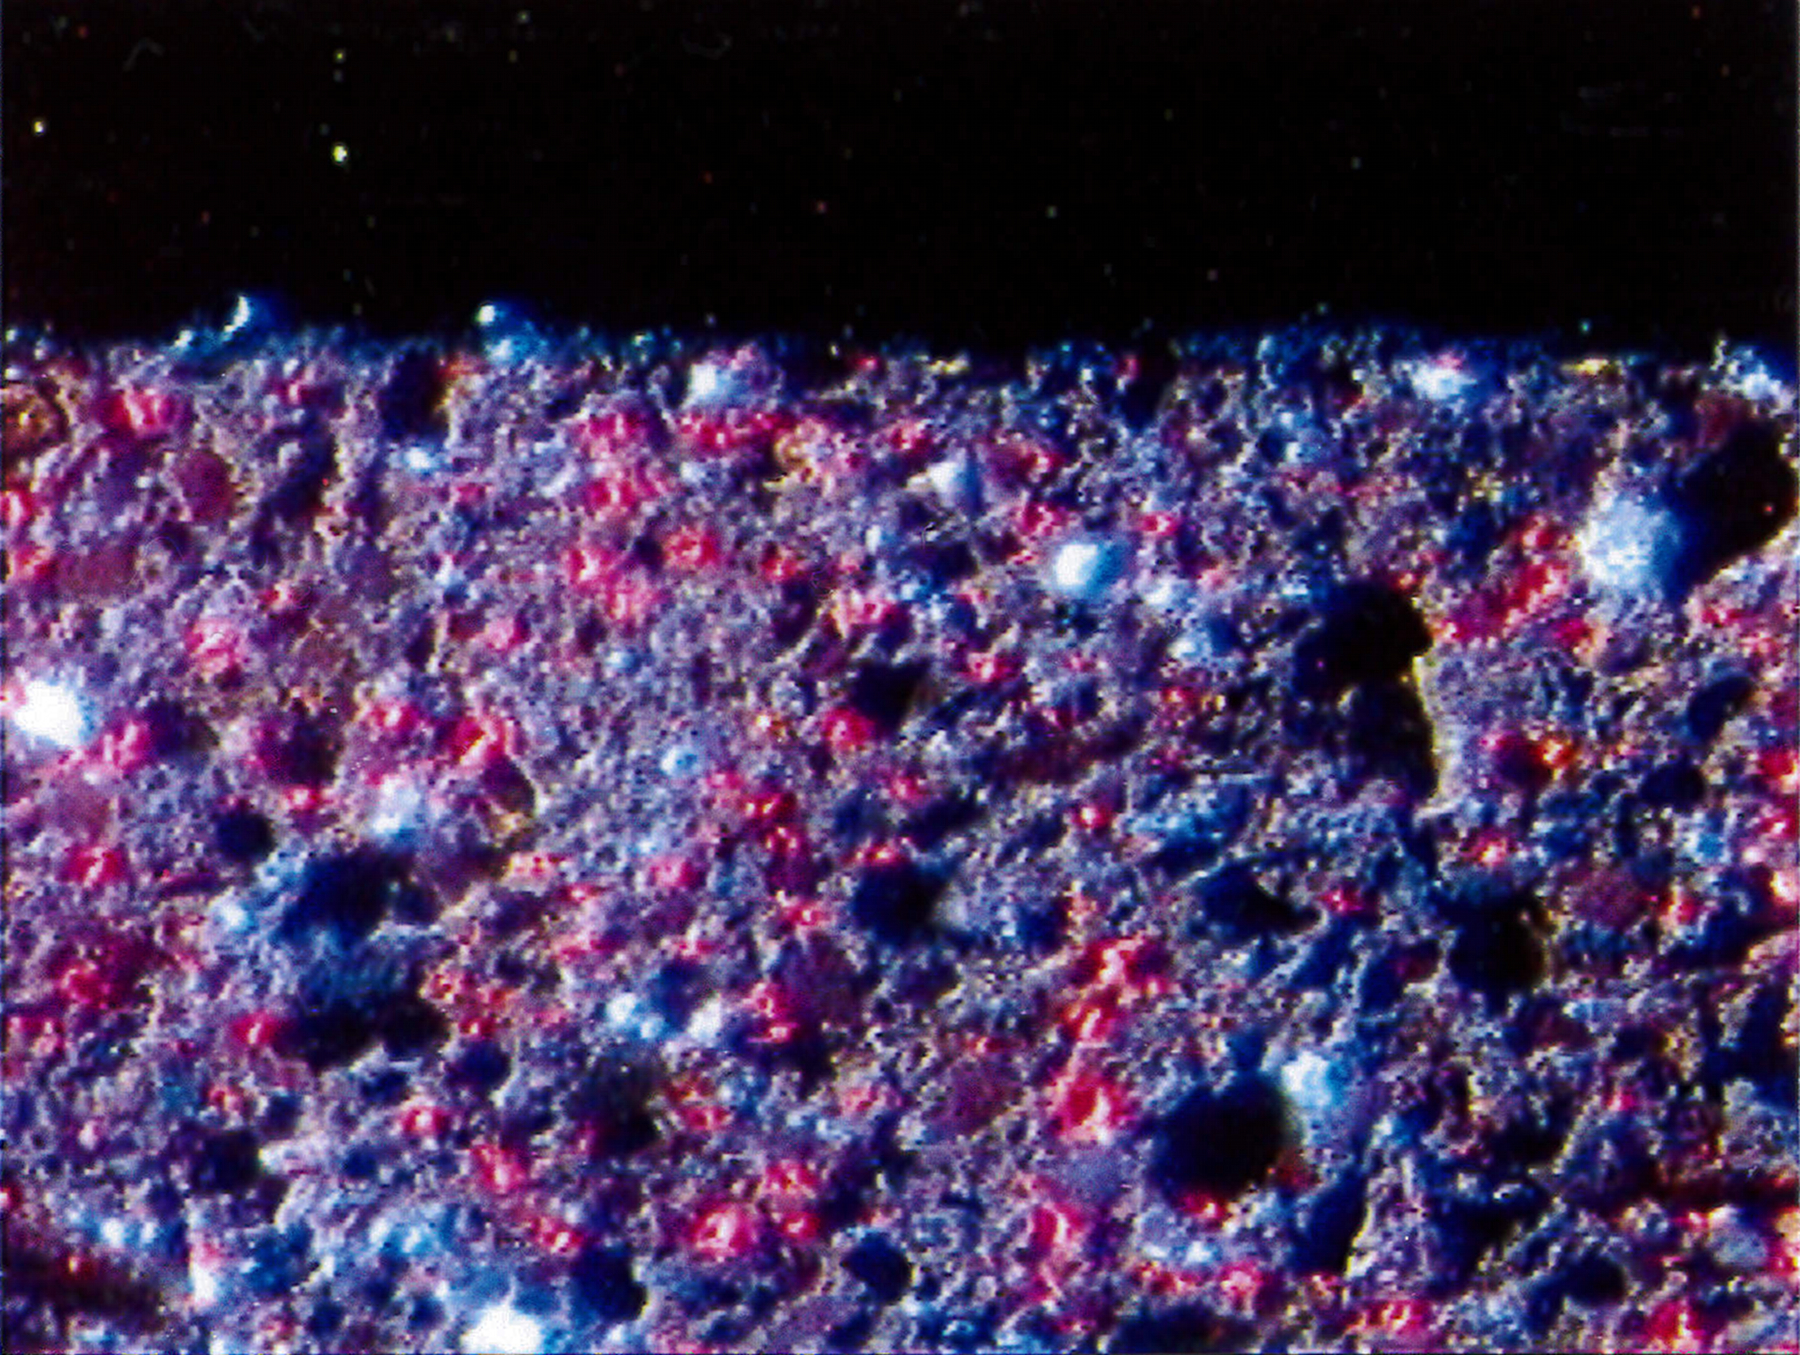
\includegraphics[width=\textwidth]{PaM_BDX6528_CL}%
    \subcaption{\CL \label{texture:6531_CL}}
  \end{minipage}
  \caption[\bdx{6531}\ -- Observation de la texture en section]
          {\legendeD.
           Observation de la texture en section 
           sur une surface de \SI{2.6x1.9}{\mm}.}
  \label{texture:6531}
\end{figure}

L'examen en section montre que la glaçure est transparente 
(\fref{texture:6531_LN}), colorée dans la masse et qu'elle 
adhère bien au support céramique. Ce dernier contient de nombreuses 
inclusions de faibles dimensions et de couleurs variées.

\subsection{Observation en \CL}
%~~~~~~~~~~~~~~~~~~~~~~~~~~~~~~~~~~~~~~~~~~~~~~~~~~~~~~~~~~~~~~~~~~~~~~
La glaçure n'est pas luminescente (\fref{texture:6531_CL}). 
On y observe des luminescences ponctuelles mauves.

La terre cuite présente une luminescence mauve à rose ainsi que 
quelques luminescences ponctuelles rouges et bleues.

On peut remarquer à l'interface glaçure-terre cuite des luminescences 
ponctuelles jaunes.

\subsection{Observation en \MEB[ie]}
%~~~~~~~~~~~~~~~~~~~~~~~~~~~~~~~~~~~~~~~~~~~~~~~~~~~~~~~~~~~~~~~~~~~~~~
La glaçure a une épaisseur moyenne de \SI{200}{\um}. Elle contient 
des cristaux non fondus de quartz (\quartz), dont la dimension peut 
aller jusqu'à \SI{100}{\um}. Ils correspondent aux émissions 
ponctuelles mauves détectées en \CL (\fref{MEB:6531_img}).

\begin{figure}[htb]
  \fakeimg{Texture au MEB, retrodiff (fig 55)}
  \caption[\bdx{6531}\ -- Observation de la texture au \MEB, 
           en mode \ERD. Ensemble glaçure/terre cuite]
          {\legendeD.
           Observation de la texture au \MEB, en mode \ERD. 
           Ensemble glaçure/terre cuite. La barre d'échelle mesure 
           \SI{200}{\um} (\zone{680x550}{\um}).}
  \label{MEB:6531_img}
\end{figure}

Une \carto de \RX de l'ensemble glaçure-terre cuite 
(\fref{MEB:6531_carto_tcgla}) montre la présence de cristaux non 
fondus de quartz (\quartz) dans la glaçure.

On observe très ponctuellement, à l'interface glaçure-terre cuite, la 
formation de cristaux de dévitrification de très petite taille. Cette 
zone semble assez riche en potassium et contient du plomb 
(\fref{MEB:6531_carto_tcgla}).

Le faible développement de cette zone d'interface laisse supposer des 
interactions faibles entre glaçure et terre cuite. L'hypothèse la plus 
probable est donc celle de l'application de la glaçure sur la terre 
cuite.

\begin{figure}[htb]
  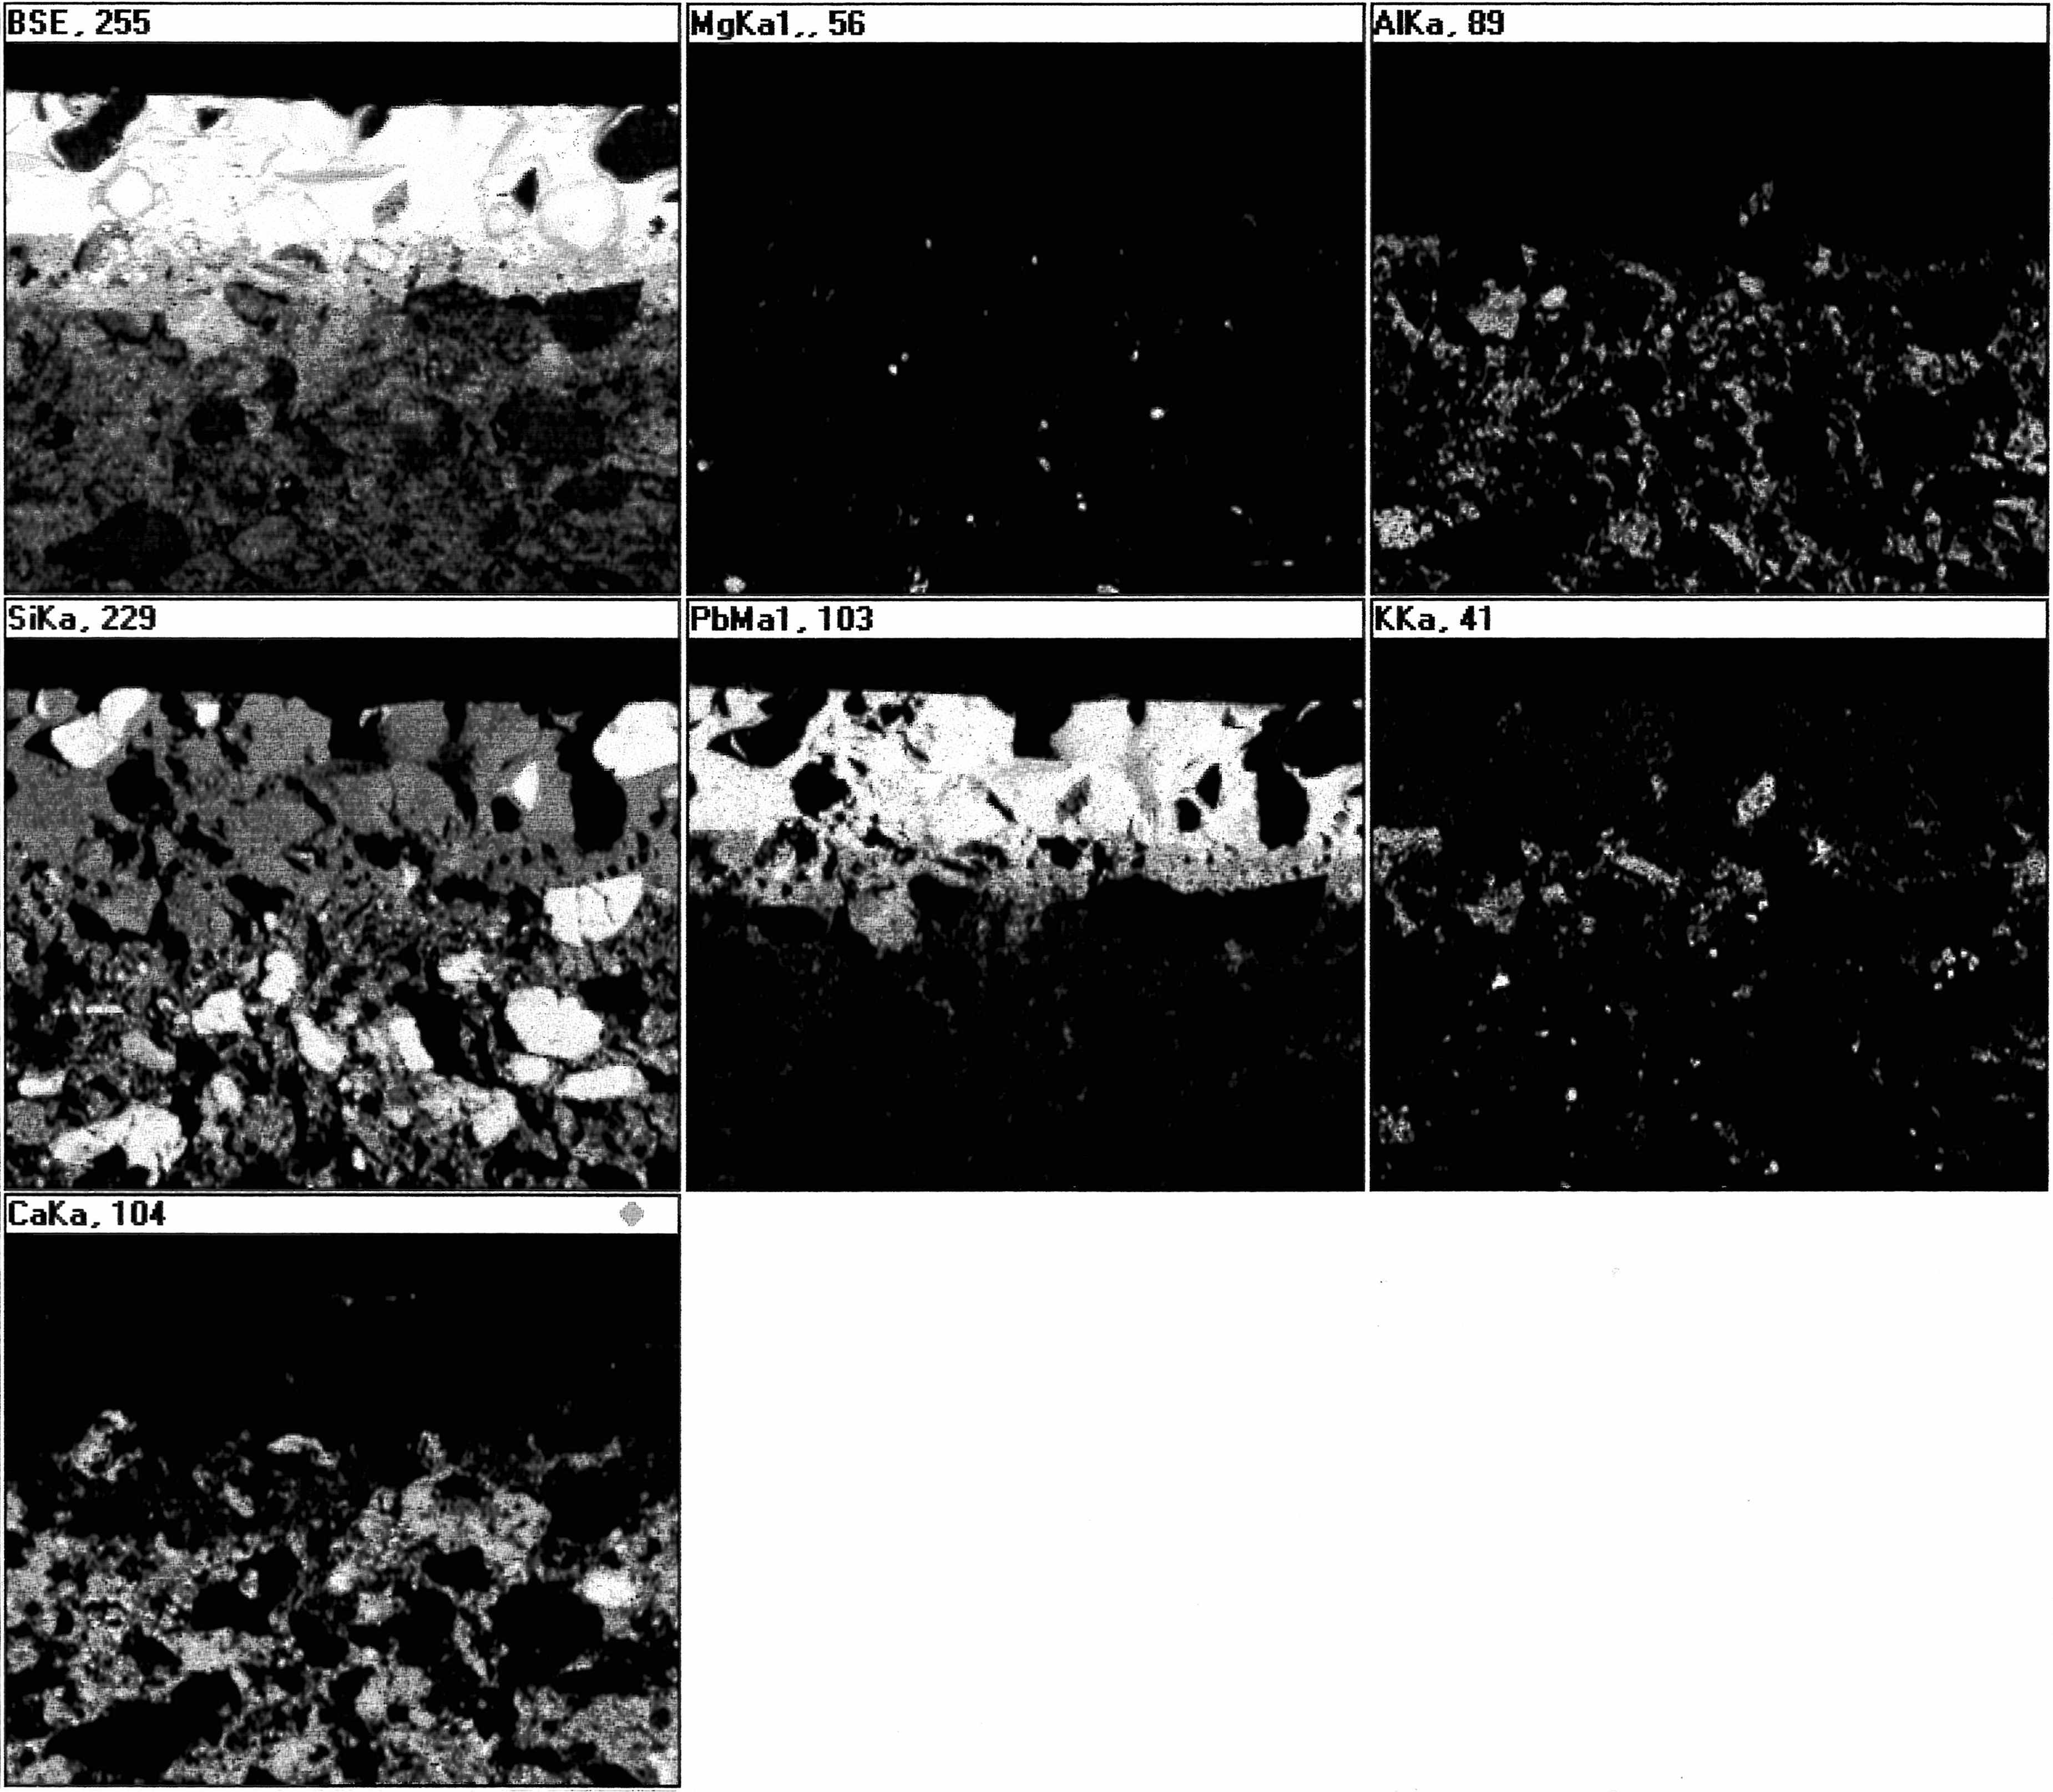
\includegraphics[width=\textwidth]{PaM_BDX6531_carto}%
  \caption[\bdx{6531}\ -- Observation de la texture au \MEB, 
           \carto de \RX de l'ensemble glaçure-terre cuite]
          {\legendeD.
           Observation de la texture au \MEB, 
           \carto de \RX de l'ensemble glaçure-terre cuite 
           (Gr=140, \zone{770x625}{\um}).}
  \label{MEB:6531_carto_tcgla}
\end{figure}

\begin{figure}[htb]
  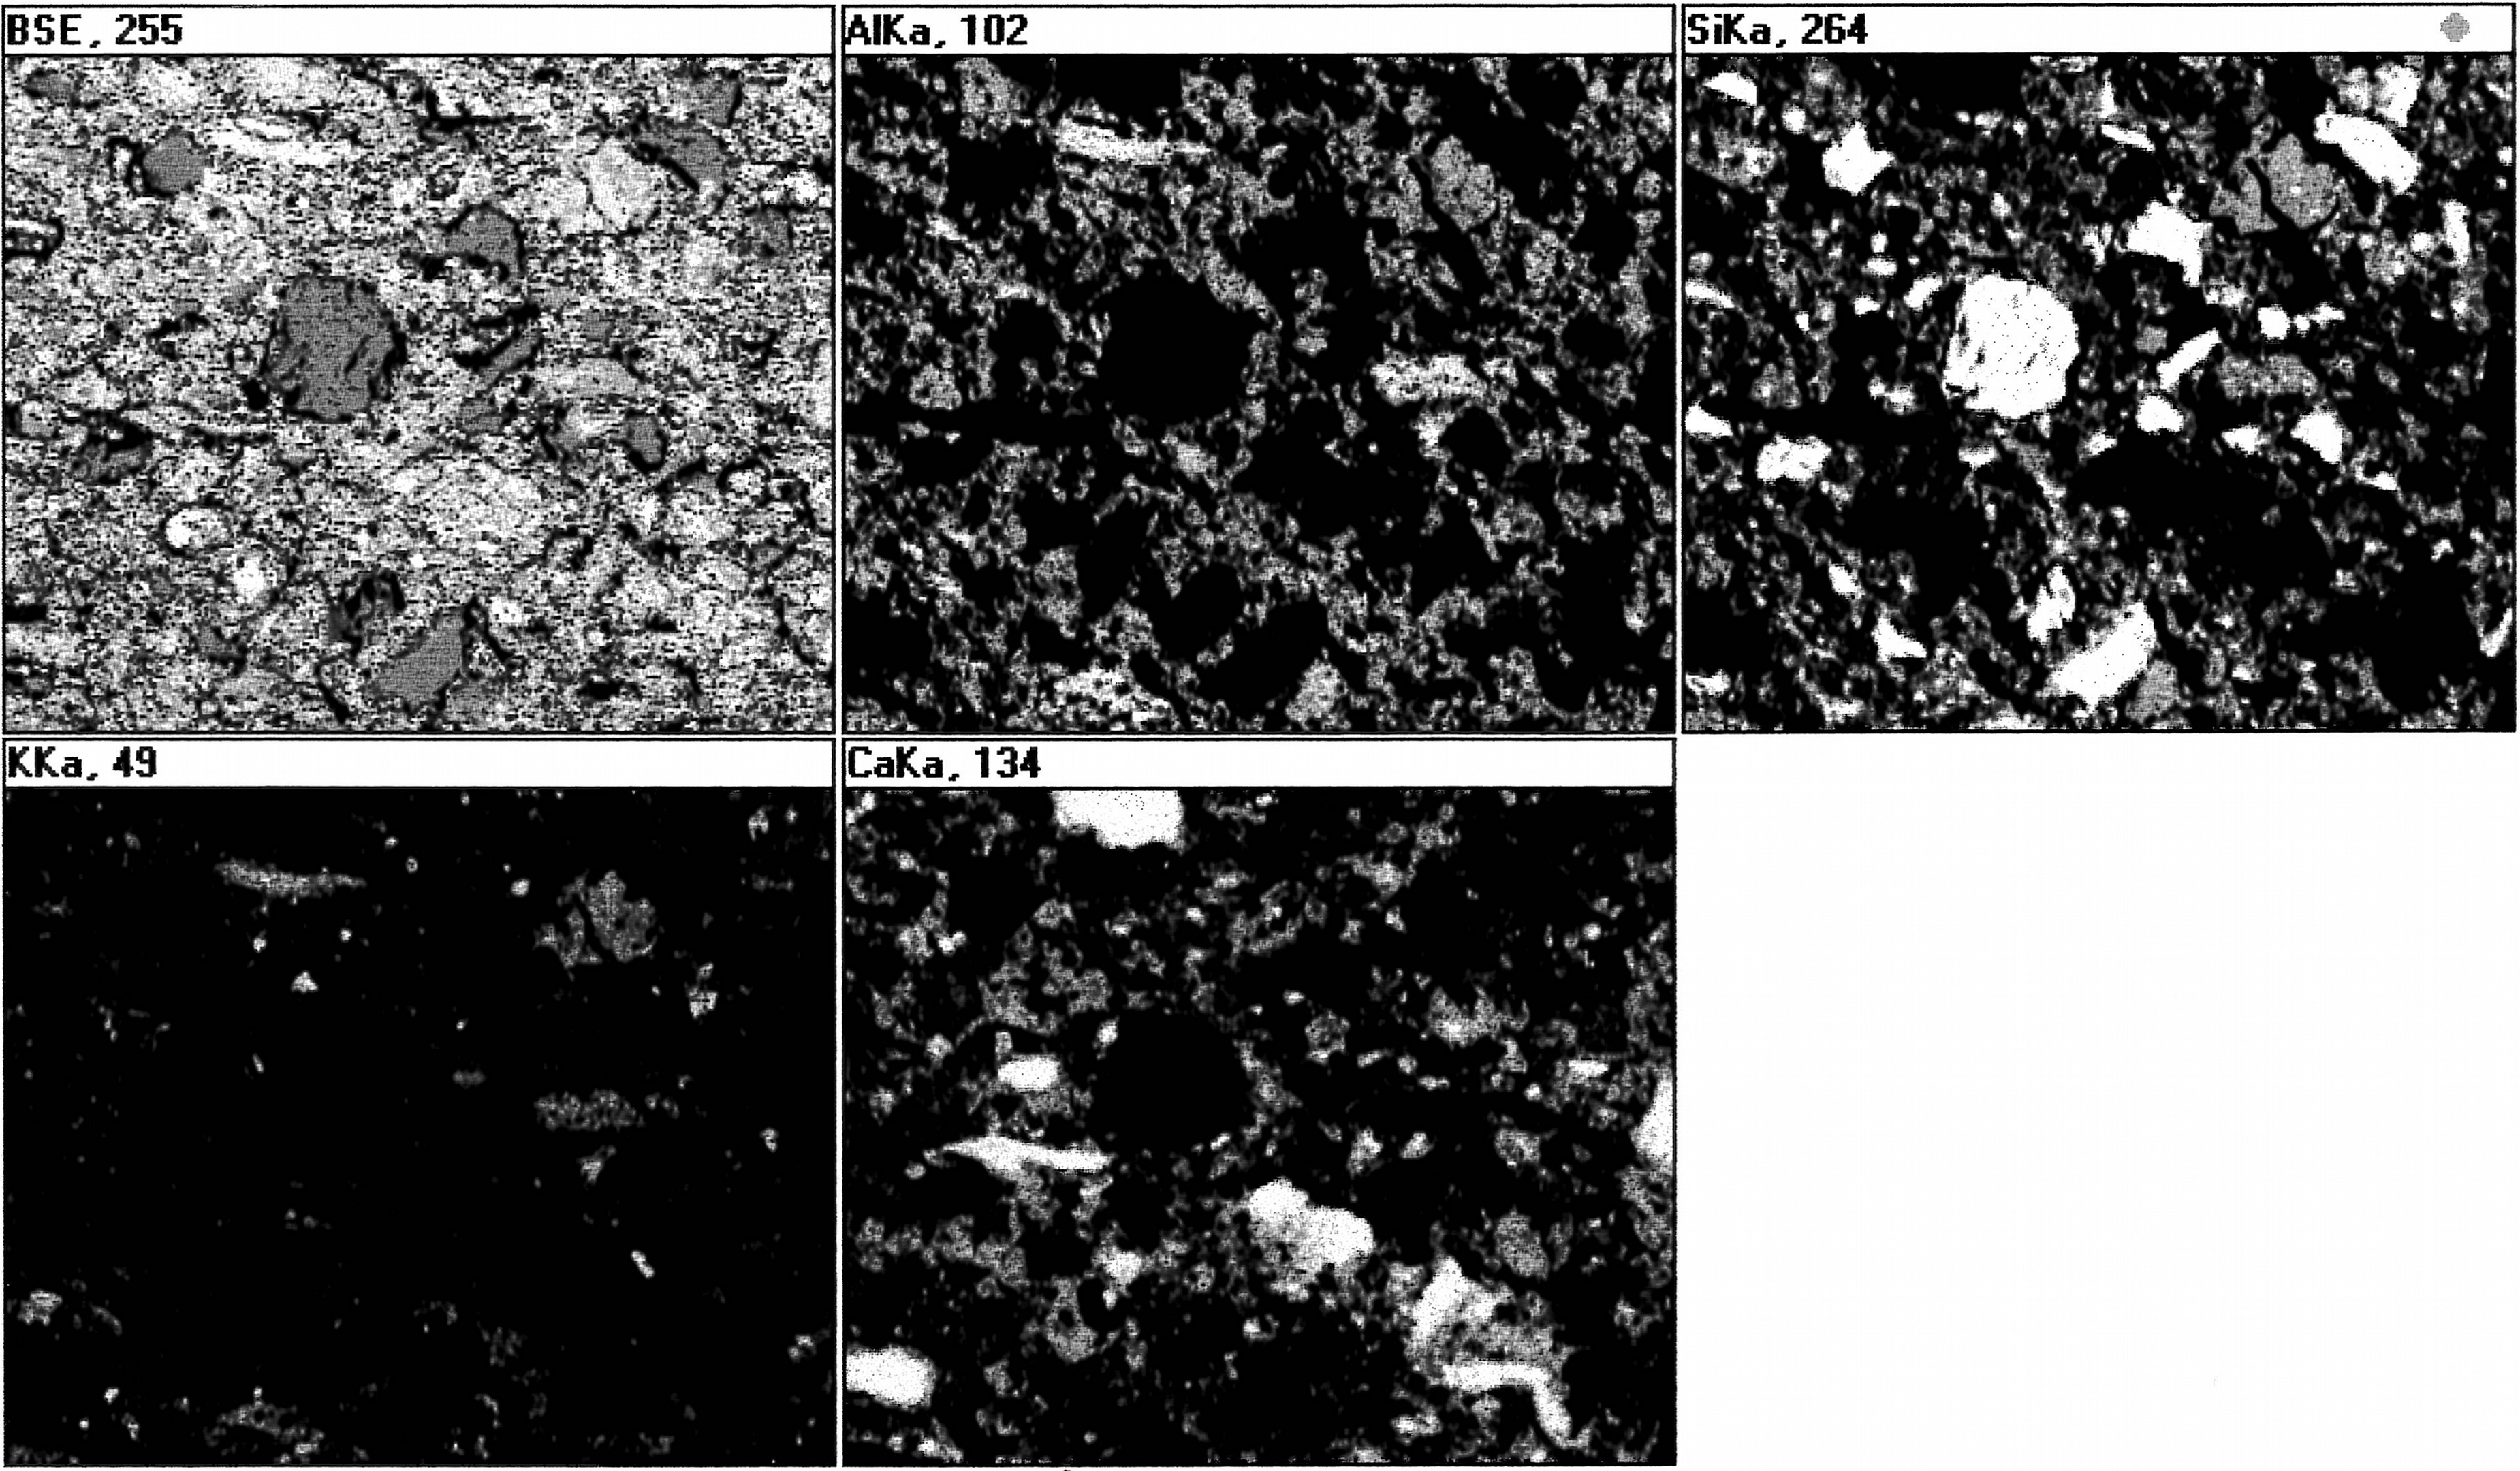
\includegraphics[width=\textwidth]{PaM_BDX6531_carto_tc}%
  \caption[\bdx{6531}\ -- Observation de la texture au \MEB, 
           \carto de \RX de la terre cuite]
          {\legendeD.
           Observation de la texture au \MEB, 
           \carto de \RX de la terre cuite 
           (Gr=140, \zone{770x625}{\um}).}
  \label{MEB:6531_carto_tc}
\end{figure}

La terre cuite contient des inclusions de quartz (\quartz), 
d'alumino-silicates potassiques ainsi que des grains d'oxydes ou de 
carbonates de calcium (\fref{MEB:6531_carto_tc}).


\section{Composition élémentaire de la glaçure}
%----------------------------------------------------------------------

\begin{table}[hbt]
  \caption[\bdx{6531}\ -- Analyse quantitative par \EDS, 
           composition élémentaire de la glaçure]
          {\legendeD. Analyse quantitative par \EDS. 
           Composition élémentaire de la glaçure miel 
           sur une surface de \SI{54x44}{\um} (\PMO).}
  \label{compelem:6531_gla}
  \begin{cartotab}
      \cartolgn{SiO2}{39.00}{1.27} &
      \cartolgn{CaO}{2.67}{0.20}   &
      \cartolgn{Al2O3}{1.04}{0.11} &
      \cartolgn{MgO}{0.39}{0.11}
    \tabularnewline
      \cartolgn{Na2O}{0.75}{0.08}  &
      \cartolgn{K2O}{1.45}{0.08}   &
      \cartolgn{Fe2O3}{3.95}{0.43} &
      \cartolgn{PbO}{50.34}{0.98}
    \tabularnewline
      \cartolgnnd{SnO2} &
      \cartolgnnd{CuO}  &
      \cartolgnnd{CoO}  &
      \cartolgnnd{MnO}
    \tabularnewline
      \cartolgnnd{Cr2O3} &
      \cartolgnnd{ZnO}   &
      \cartolgnnd{Sb2O3} &
      \cartolgn{TiO2}{0.19}{0.02}
    \tabularnewline
      \cartolgnnd{S}            &
      \cartolgnnd{P2O5}         &
      \cartolgn{Cl}{0.20}{0.09} &
      \cartolgnnd{As2O3}
    \tabularnewline
  \end{cartotab}
\end{table}

Il s'agit d'une glaçure plombifère non opacifiée 
(\tref{compelem:6531_gla}). C'est le fer, sous la forme~\ch{Fe^3+}, 
qui lui donne sa coloration miel.


\section{Étude de la terre cuite support}
%----------------------------------------------------------------------

\subsection{Composition élémentaire}
%~~~~~~~~~~~~~~~~~~~~~~~~~~~~~~~~~~~~~~~~~~~~~~~~~~~~~~~~~~~~~~~~~~~~~~
\begin{table}[hbt]
  \caption[\bdx{6531}\ -- Analyse quantitative par \EDS, 
           composition élémentaire de la terre cuite]
          {\legendeD. Analyse quantitative par \EDS. 
           Composition élémentaire de la terre cuite 
           sur une surface de \SI{1080x876}{\um} (\PMO).}
  \label{compelem:6531_tc}
  \begin{cartotab}
      \cartolgn{SiO2}{60.58}{4.99}  &
      \cartolgn{CaO}{17.68}{1.82}   &
      \cartolgn{Al2O3}{10.93}{1.68} &
      \cartolgn{MgO}{2.33}{0.17}
    \tabularnewline
      \cartolgn{Na2O}{0.45}{0.09}  &
      \cartolgn{K2O}{1.46}{0.25}   &
      \cartolgn{Fe2O3}{5.65}{1.00} &
      \cartolgnnd{PbO}
    \tabularnewline
      \cartolgnnd{SnO2} &
      \cartolgnnd{CuO}  &
      \cartolgnnd{CoO}  &
      \cartolgnnd{MnO}
    \tabularnewline
      \cartolgnnd{Cr2O3} &
      \cartolgnnd{ZnO}   &
      \cartolgnnd{Sb2O3} &
      \cartolgn{TiO2}{0.60}{0.09}
    \tabularnewline
      \cartolgn{S}{0.33}{0.03} &
      \cartolgnnd{P2O5}        &
      \cartolgnnd{Cl}          &
      \cartolgnnd{As2O3}
    \tabularnewline
  \end{cartotab}
\end{table}

La terre cuite est riche en calcium (\tref{compelem:6531_tc}). C'est 
le \ch{Fe^3+} en atmosphère de cuisson oxydante qui lui donne sa 
coloration ocre rosé \autocite{Echallier_1984}.

\subsection{Composition \cristallo}
%~~~~~~~~~~~~~~~~~~~~~~~~~~~~~~~~~~~~~~~~~~~~~~~~~~~~~~~~~~~~~~~~~~~~~~
\begin{figure}[htb]
  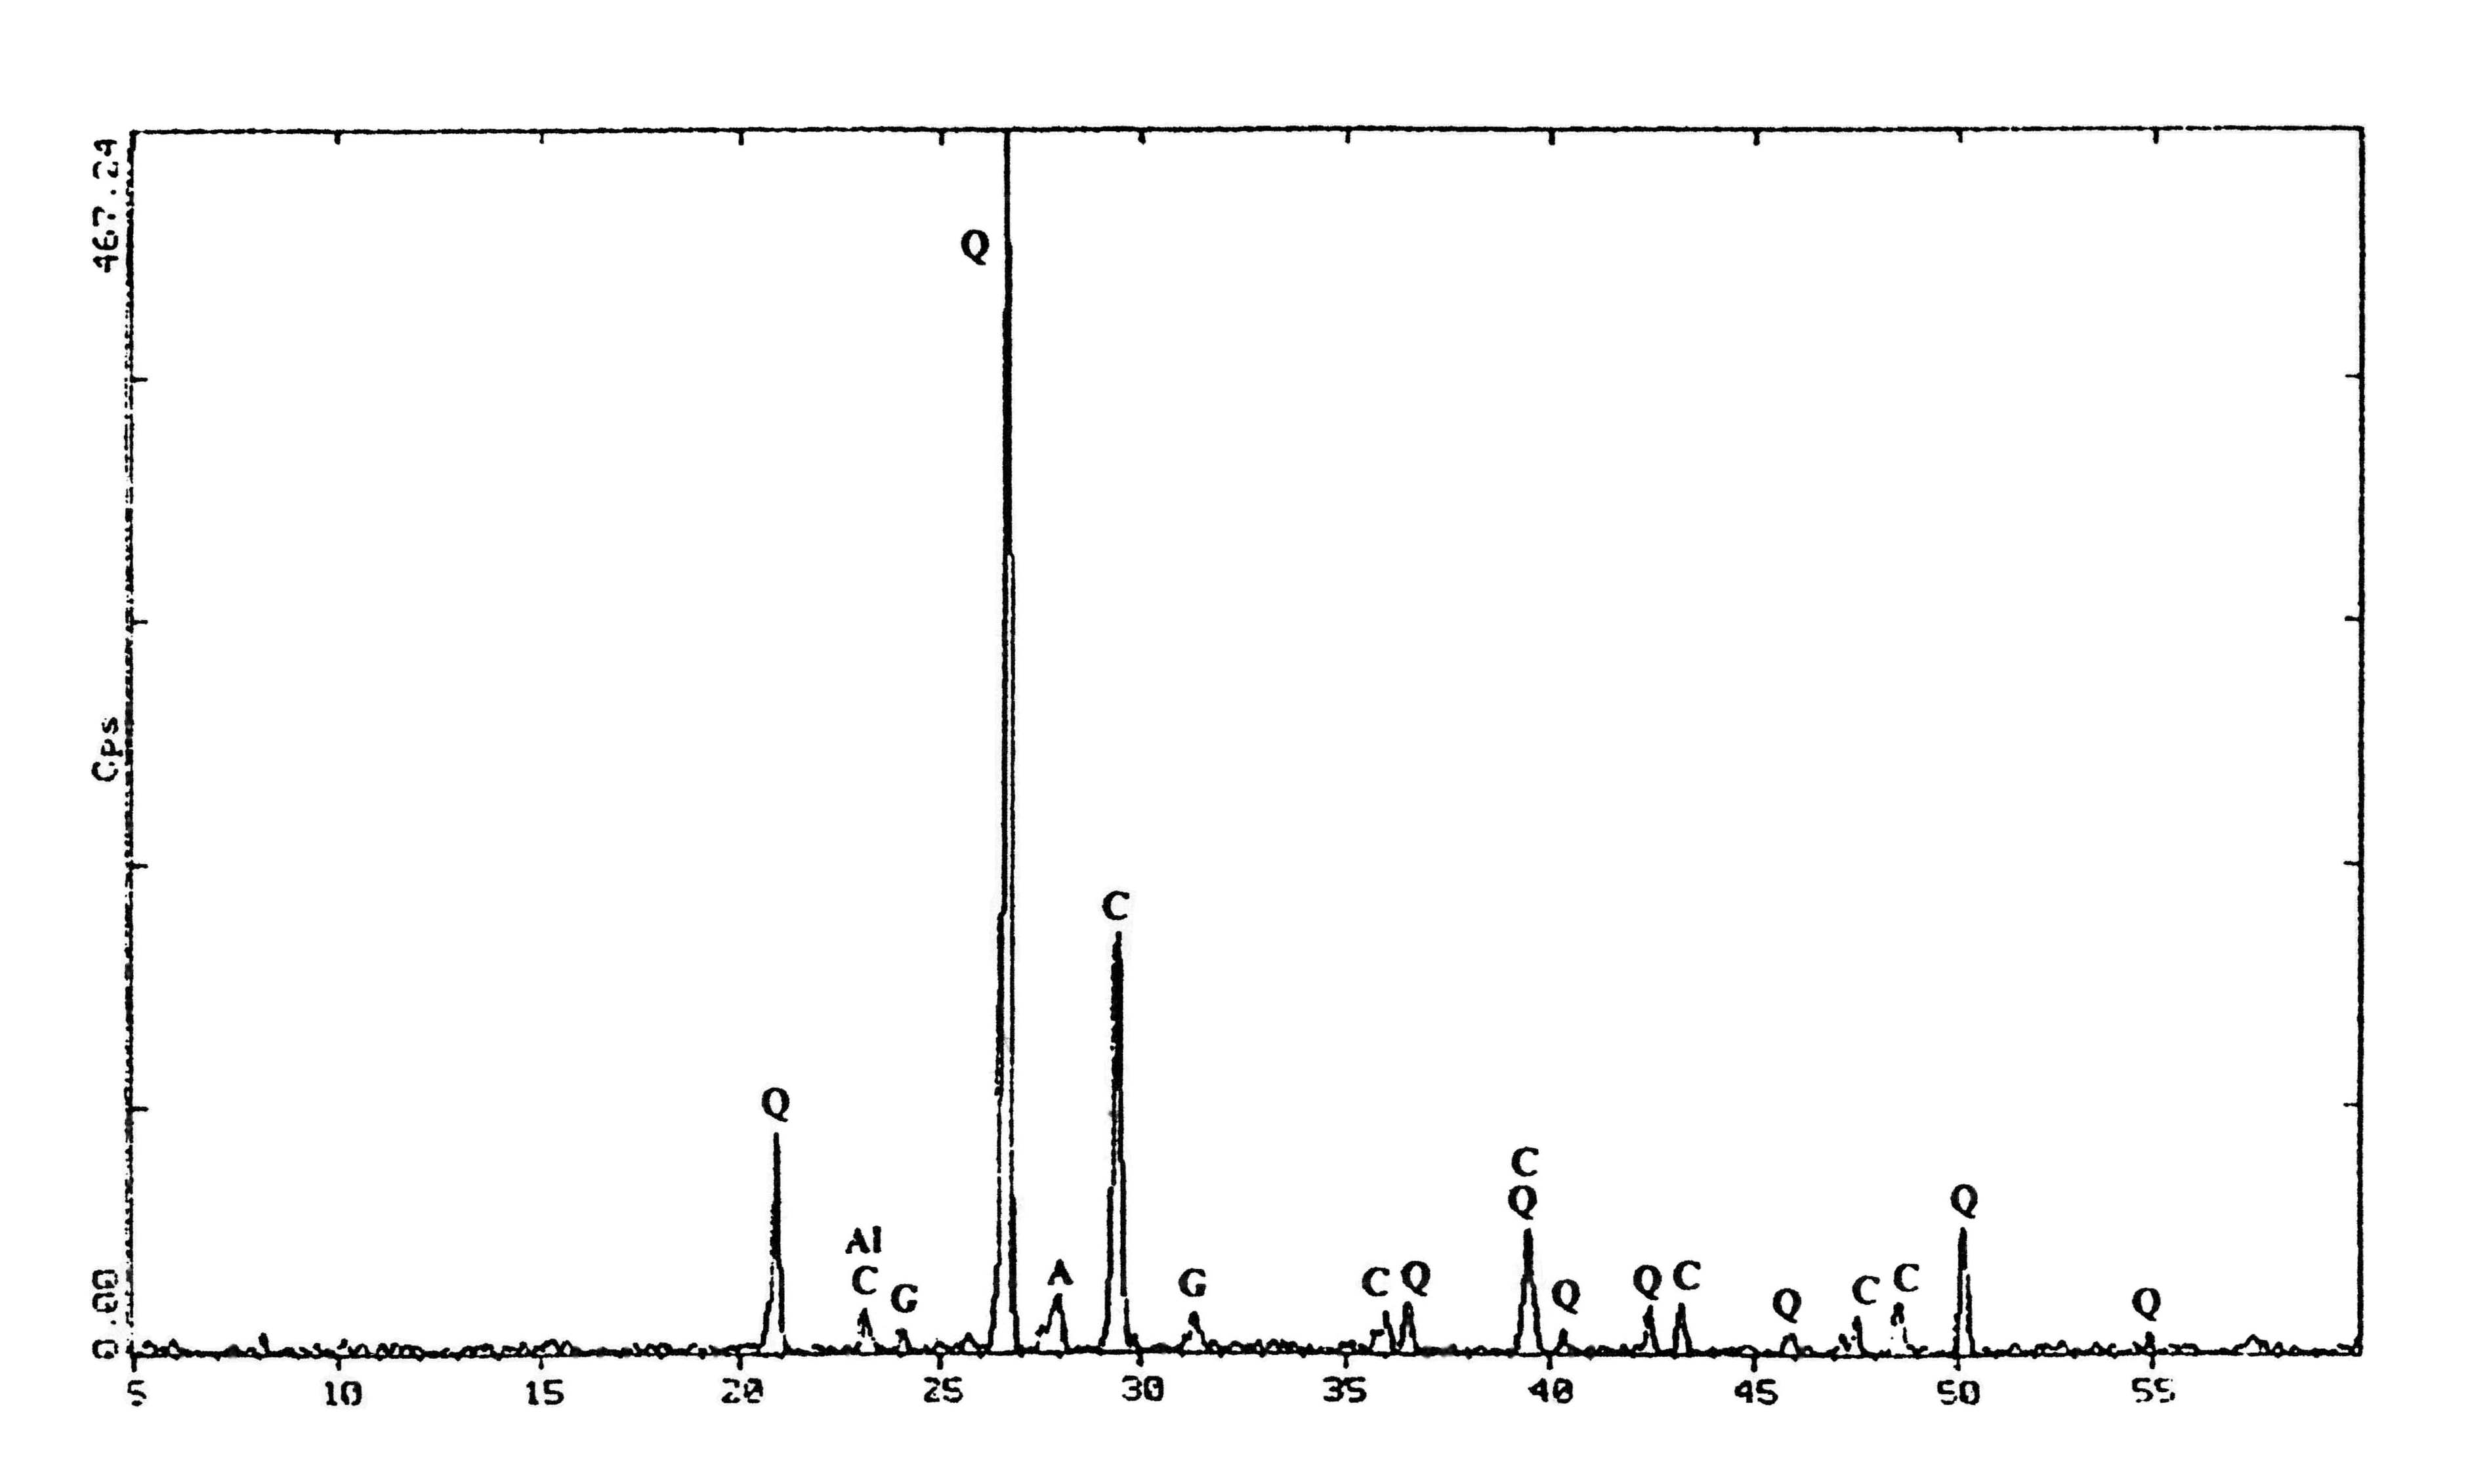
\includegraphics[width=\textwidth]{PaM_BDX6531_DX}
  \caption[\bdx{6531}\ -- Diffraction de \RX sur poudre 
           de la terre cuite]
          {\legendeD.
           \DX[D] sur poudre de la terre cuite. 
           Mise en évidence de la présence de quartz (Q), 
           calcite (C), albite (Al), gehlénite (G), anorthite (A).}
  \label{DRX:6531}
\end{figure}

Le principal composé cristallisé mis en évidence par \DX sur poudre 
(\fref{DRX:6531}) est le quartz (\quartz). On relève également la 
présence, à des teneurs plus faibles, de calcite (\calcite) pouvant 
correspondre aux émissions rouges détectées en \CL, de gehlénite 
(\gehlenite) et, probablement d'albite (\albite) et d'anorthite 
(\anorthite). La très faible intensité des raies de ces derniers en 
rend l'indexation incertaine. Les feldspaths calciques peuvent être 
responsables des émissions bleues détectées en \CL.

La gehlénite et l'anorthite sont deux phases se développant à 
haute température. Leur présence laisse supposer que la température 
de cuisson de la pâte céramique a atteint 
\SIrange[range-phrase=\ à\ ]{850}{900}{\degC} \autocite{Peters_1978}.


\section{Sur la présence et l'identification de cristaux de 
         dévitrification}
%----------------------------------------------------------------------

On distingue, dans la zone d'interface terre cuite-glaçure, des 
cristaux de forme aciculaire. Ce sont des cristaux de dévitrification 
dont la composition élémentaire n'a pu être déterminée étant données 
leurs faibles dimensions.


\section{Étude des altérations de la glaçure}
%----------------------------------------------------------------------

Aucune figure d'altération n'a été mise en évidence dans la glaçure, 
ni visuellement, ni en \MEB[ie] (MEB).


\section{Bilan}
%----------------------------------------------------------------------

Cet échantillon est donc une pièce de céramique portant une glaçure 
plombifère dont la coloration miel est due au \ch{Fe^3+} en atmosphère 
de cuisson oxydante.

Son support de terre cuite est de type calcique. Sa coloration 
ocre-rose est due à la présence de \ch{Fe^3+} en atmosphère de 
cuisson oxydante.

Sa composition \cristallo (quartz, calcite, albite, gehlénite, 
anorthite) laisse penser qu'elle a été cuite à une température de 
l'ordre de \SIrange[range-phrase=\ à\ ]{850}{900}{\degC}.

À l'interface glaçure-terre cuite, on distingue des luminescences 
ponctuelles jaunes, associées à la présence de cristaux de 
dévitrification dont les faibles dimensions n'ont pas permis de 
déterminés la composition élémentaire. Le faible développement de 
cette zone laisse envisager l'application du mélange glaçurant sur 
une terre cuite.

La glaçure ne présente pas de figure d'altération d'origine chimique 
mais une usure mécanique de surface.
